\section{Dictionaries and Tolerant Retrieval}\label{ch4}
In Chapters \ref{ch2} and \ref{ch3} we developed the ideas underlying inverted indexes for handling Boolean and proximity queries, so now we develop techniques that are robust to typographical errors in the query, as well as alternative spellings (tolerant retrieval).

In section \ref{4.1} we develop data structures that help the search of terms in the vocabulary in an inverted index, in Section \ref{4.2} we study the idea of \textit{wildcard queries}, that are used when the user is uncertain of the spelling of a query term, while in Section \ref{4.3} we focus on spelling errors.

\subsection{Search structures for dictionaries}\label{4.1}
Given an \textbf{inverted index} and a \textbf{query}, our first task is to determine whether each query term exists in the vocabulary and if so, identify the pointer to the corresponding postings. This operation is usually implemented by exploiting the \textbf{vocabulary} data structure: in our case, the dictionary stores the term vocabulary (representing the \textit{keys} of the dictionary), its document frequency and the pointer to the corresponding posting list. Usually, a vocabulary is implemented by using \textbf{hash tables} or \textbf{search trees}, and the choice between the two solutions depend on many factors, for example the number of keys that we have, whether this number is likely to change or not, the relative frequencies of each key etc..

\subsubsection{Hash Tables}
In the \textbf{hashing} technique, each vocabulary term is hashed into an integer (we assume that this operation minimizes the collisions), which is then used to access the corresponding posting list. The main \textbf{advantage} of this solution is that the vocabulary lookup is very fast, $O(1)$. However, there are several \textbf{disadvantages}: the hash table does not provide an easy way to find minor variants of the term, since different terms results in two different integers, and does not allow to search for a term using the prefix (tolerant retrieval). Finally, one important issue is that if the vocabulary keeps growing, a re-hashing operation of the whole vocabulary must be done, and this is usually very expensive.

\subsubsection{Search Trees}
\textbf{Search trees} are data structures that overcome some of the issues of the hash tables. The best-known search tree is the \textit{binary tree}, in which each internal node has two children, and it can be considered as a binary test that affects the search for a term, in the sense that the outcome of the test determines one of the two sub-trees along which the search proceeds. Picture \ref{binary tree} gives an example of binary tree used for a dictionary.

\begin{figure}[h!]
		\centering
		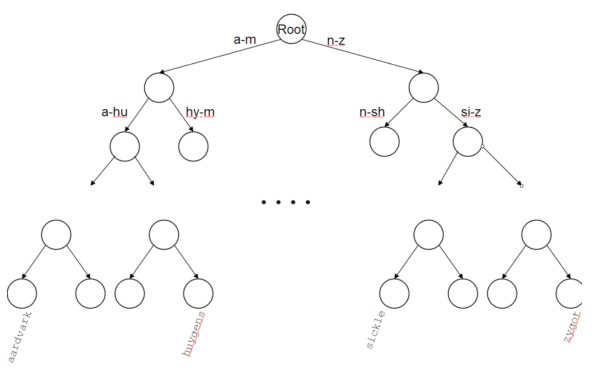
\includegraphics[scale = 1.8]{img/binary tree.jpg}
		\label{binary tree}
        \caption{Binary tree for a dictionary}
\end{figure}

The main issue about binary trees is that in order to implement efficient search, i.e. with complexity $O(logM)$, the tree must be \textbf{balanced}, so a big disadvantage of this structure is given by the overhead of maintaining the tree balanced when a new document is inserted.

To overcome this problem, usually the \textbf{B-tree} data structure is used: the \textit{B-tree} is a generalization of the binary tree in which every internal nodes has a number of children in the interval $[a,b]$, where $a$ and $b$ are appropriate natural numbers. Picture \ref{b tree} shows a B-tree where $a = 2$ and $b = 4$. We notice that, because a range of child nodes is permitted, B-trees do not need re-balancing as frequently as binary trees, but on the other hand they may waste more space when the nodes are not entirely full.

\begin{figure}[h!]
		\centering
		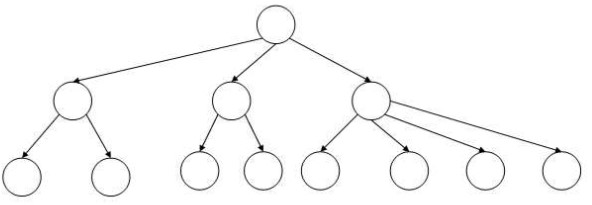
\includegraphics[scale = 1.8]{img/b tree.jpg}
		\label{b tree}
        \caption{B-tree for a dictionary}
\end{figure}

In general, the simplest search tree to implement is the \textit{binary tree}, but \textit{B-trees} are the most used. We notice that trees, unlike hash tables, require a \textbf{standard ordering} of the characters, which is usually represented by the \textit{lexicographic order}. The \textbf{advantage} of using the \textit{search trees} is that they solve the prefix problem, i.e. they allow to search for a term by providing its prefix. The \textbf{disadvantages} are that they are usually slower than hash tables ($O(log M)$ vs $O(1)$), and they may require the re-balancing operation, which is quite expensive, although the B-trees mitigate this problem.

\subsection{Wildcard queries}\label{4.2}
As we introduced before, the wildcard queries can be used when the user is uncertain of the spelling of a query, or when the user wants to retrieve documents containing all the variants of a term etc..

An example of wildcard query is \textit{mon*}, and it is called \textbf{trailing wildcard query}, since the symbol * occurs only once at the end of the string. This type of wildcard query is quite simple to be answered by using a binary tree (or B-tree) lexicon, since we have to search for all the words s.t. $\text{mon} \leq \text{word} \leq \text{moo}$, by traversing the tree.

A slight generalization of this typology is the \textbf{leading wildcard query}, where the queries are in the form \textit{*mon}: these queries can be answered by maintaining an additional reverse B-tree that stores the terms backwards.

Finally, we can handle an even more general case: wildcard queries in which there is a single * in the middle of the query, such as \textit{co*tion}. To solve these queries, we use the regular B-tree to retrieve the set of terms beginning with the prefix \textit{co}, then we use the reverse B-tree to retrieve the set of terms ending with the suffix \textit{tion}, and finally we intersect the two term sets using the standard inverted index. Obviously, this solution is quite expensive, and for this reason a possible improvement can be brought by transforming the wildcard queries so that the *'s occur always at the end of the terms. This approach gives rise to the \textbf{permuterm index}.

\subsubsection{Permuterm index}
The \textbf{permuterm index} is a form of inverted index in which all the possible permutations of a term all link to the original vocabulary term, as represented in Picture \ref{permuterm_index}. Notice that the character \$ is a special symbol that marks the end of a term: this character increases the vocabulary size, since we now store $n+1$ terms, where $n$ is the term size, rather than just 1. The set of rotated terms in the permuterm index is called \textit{permuterm vocabulary}.

\begin{figure}[h!]
		\centering
		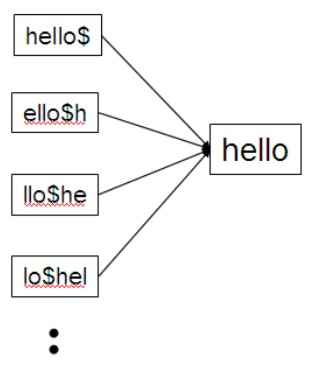
\includegraphics[scale = 1.6]{img/permuterm index.jpg}
		\label{permuterm_index}
        \caption{A portion of a permuterm index}
\end{figure}

As we introduced before, the goal of the \textit{permuterm index} is to rotate the wildcard query so that the * symbol appears at the end of the string. For example, if the query is \textit{h*e}, we insert the symbol \$, so \textit{h*e\$}, and our goal is to consider the term \textit{e\$h*}. Finally we can search the terms starting with \textit{e\$h*} using a standard B-tree lookup to retrieve the matching documents.

Now the problem is how to handle wildcard queries containing multiple * symbols, such as \textit{fi*mo*er}.  In this case we first enumerate the terms in the dictionary that are in the permuterm index of \textit{er\$fi*}. Not all such dictionary terms will have the string \textit{mo} in the middle, so we filter these out by exhaustive enumeration, checking each candidate to see if it contains \textit{mo}. Finally, we run the surviving terms through the standard inverted index for document retrieval.

One \textbf{disadvantage} of the permuterm index is that its dictionary becomes like 4 to 10 times larger than the original one, so we now introduce another method to answer wildcard queries.

\subsubsection{$k$-gram indexes for wildcard queries}
A $k$-gram is a sequence of $k$ characters, so \textit{cas}, \textit{ast} and \textit{stl} are all 3-grams occurring in the term \textit{castle}. We use a special character \$ to denote the beginning or end of a term, so the full set of 3-grams generated for castle is: \textit{\$ca}, \textit{cas}, \textit{ast}, \textit{stl}, \textit{tle}, \textit{le\$}. 

In the \textit{$k$-gram index}, the vocabulary contains all the $k$-grams that occur in any term in the vocabulary, and each postings list of a $k$-gram contains all the terms containing the corresponding $k$-gram. An example is provided in Picture \ref{kgram}.

\begin{figure}[h!]
		\centering
		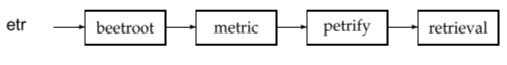
\includegraphics[scale = 1.6]{img/k-grams .jpg}
		\label{kgram}
        \caption{Postings list of a $k$-gram}
\end{figure}

Now, this particular index can be used for solving wildcard queries in the following way: suppose that the query is \textit{re*ve}, we then run the Boolean query \textit{\$re} AND \textit{ve\$}, and each of the matching terms is then looked up in the standard inverted index to yield documents matching the query. However, this approach leads to the retrieval of some \textbf{false positives}. Consider for example the query \textit{red*}: following the approach described above, we would perform the Boolean query \textit{\$re} AND \textit{red}, but this would lead to match terms like \textit{retired}, which is a false positives w.r.t. the original query. In this sense, a \textbf{post-processing} phase must be introduced, in order to filter the false positives against the original query: the surviving terms are then looked up in the standard inverted index.

\subsubsection{Permuterm index vs $k$-gram index}
As we said before, \textbf{permuterm index} is not space efficient: if $n$ is the average length of a word, using the character \$ as a suffix, we add $n$ rotations to the vocabulary; overall, we need $(n+1) * (n+1)$ chars for a term of $n$ chars.

With 2-grams, considering the leading and trailing \$, we use $(n+1) * 2$ chars, where $n+1$ is the number of bigrams for each term considering the symbol \$. Finally, with 3-grams we need $n*3$ chars.

In general, wildcard queries can result in very expensive query execution, and for this reason this capability is hidden behind an interface (say "Advanced Query"), which most users do not use.

\subsection{Spelling correction}\label{4.3}
We now consider the problem of \textbf{spelling correction} in queries, and in particular we focus on two possible solutions: the first one is based on \textit{edit distance}, while the second one on \textit{k-gram overlap}.

In general, the two main uses of the spelling correction are:

\begin{itemize}
    \item correcting the documents being indexed, and in particular this in important if the documents are retrieved using OCR (optical character recognition);
    \item correcting user queries to retrieve the correct answers (\textit{Did you mean..?}).
\end{itemize}

\subsubsection{Forms of spelling correction}
We focus on two specific forms of spelling correction:

\begin{itemize}
    \item \textbf{isolated-term correction}, in which we attempt to correct a single query term at a time. This type of correction does not catch typos resulting in correctly spelled words, e.g. \textit{flew form Heathrow}, since each term in the query is correctly spelled in isolation;
    \item \textbf{context-sensitive correction}, in which the surrounding words are considered. In this case, the mispelling of the previous example is detected.
\end{itemize}

In general, given a lexicon and a char sequence $Q$, the goal of this technique is to return the words in the lexicon closest to $Q$, and, in particular, among alternative correct spellings for a mis-spelled query, choose the "nearest" one. If two correctly spelled queries are tied, then select the most common.

\textbf{\underline{Isolated-term correction}}

We first analyze two techniques for addressing isolated-term correction: edit distance and $k$-gram overlap. 

Given two strings $S_1$ and $S_2$, the \textit{edit distance} (or \textit{Levenshtein distance}) is the minimum number of edit operations to convert one to the other. The operations are typically character-level, and they're usually \textit{insert}, \textit{delete}, \textit{replace} and \textit{transposition}. For example, the \textit{edit distance} between \textit{cat} and \textit{act} is 2, since two replacements are needed. A more accurate measure can be also obtained using the \textit{weighted edit distance}, where different weights are used for different kind of edit operations, depending on the likelihood of letters that are replaced (e.g. $m$ is more likely to be mis-typed as $n$ than as $q$, so replacing $m$ by $n$ is a smaller edit disance than by $q$). In general, the (weighted) edit distance can be computed using dynamic programming with complexity $O(|S_1| \text{x} |S_2|)$, and in the case of the weighted version, a weight matrix must be provided as input to the algorithm.

The spelling correction problem however demands more than computing edit distance: given a set $S$ of strings (corresponding to terms in the vocabulary) and a query string $q$, we seek the string(s) in $V$ of least edit distance from $q$. The obvious way of doing this is to compute the edit distance from $q$ to each string in $V$, before selecting the string(s) of minimum distance: however, this naive solution is quite expensive and extremely slow ($O(n^2)$). For this reason, some heuristics are adopted to cut the set of candidate dictionary terms: 

\begin{itemize}
    \item restrict the search to dictionary terms beginning with the same letter as the query string: in this case we hope that spelling errors do not occur in the first letter of the query;
    \item generate everything up to edit distance $k = 1,2$ and then intersect these candidates with terms in the index lexicon.
\end{itemize}

Another way to limit the set of vocabulary terms for which we compute edit distances to the query term is by using the \textbf{$k$-gram index} that we introduced for wildcard queries. In particular, this index is used to retrieve vocabulary terms that have many $k$-grams in common with the query: for example, the bigram index in Picture \ref{kgram_spelling} shows the postings for the three brigrams of the word \textit{bord}. Suppose that we want to retrieve the vocabulary terms that contain at least two of these bigrams, then a single scan of the postings would result in retrieving \textit{aboard}, \textit{border}, and \textit{boardroom}.

\begin{figure}[h!]
		\centering
		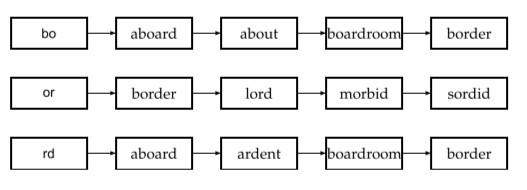
\includegraphics[scale = 1.6]{img/kgram spelling.jpg}
		\label{kgram_spelling}
        \caption{$k$-gram for spelling correction}
\end{figure}

However, we would like to consider a more precise measure of overlap, and one option could be the \textit{Jaccard coefficient}, which is defined as $\frac{|A \cap B|}{|A \cup B|}$, where $A$ and $B$ are, respectively, the set of $k$-grams in the query and the set of $k$-grams in a vocabulary term. As the scan proceeds, we proceed from one vocabulary term $t$ to the next, computing on the fly the \textit{Jaccard coefficient} between $q$ and $t$. If the coefficient exceeds a preset \textbf{threshold}, we add $t$ to the output; if not, we move on to the next term in the postings.

\underline{\textbf{Context-sensitive approach}}

As we underlined before, isolated-term correction would fail to correct typographical errors such as \textit{flew form Heathrow}, where all three query terms are correctly spelled: our desired output would be that the search engine may offer the corrected query \textit{few from Heathrow}. 

The simplest way to do this is to enumerate corrections of each of the three query terms (using the methods we described before) even though each query term is correctly spelled, then try substitutions of each correction in the phrase. For the example \textit{flew form Heathrow}, we enumerate such phrases as \textit{fled form Heathrow} and \textit{flew fore Heathrow}. For each such substitute phrase, the search engine runs the query and determines the number of matching results: finally, the engine suggests the alternative that has lots of hits. Obviously, this enumeration can be expensive if we find many corrections of the individual terms, since we could encounter a large number of combinations of alternatives.

A possible heuristic that can be used for reduce the search space is to retain only the most frequent combinations in the collection or in the query logs, which contain previous queries by the users. For example, we would retain \textit{flew from} as an alternative to try and extend to a three-term corrected query, but perhaps not \textit{fled fore} or \textit{flea form}.

